% Created by tikzDevice version 0.12 on 2019-09-25 16:08:43
% !TEX encoding = UTF-8 Unicode
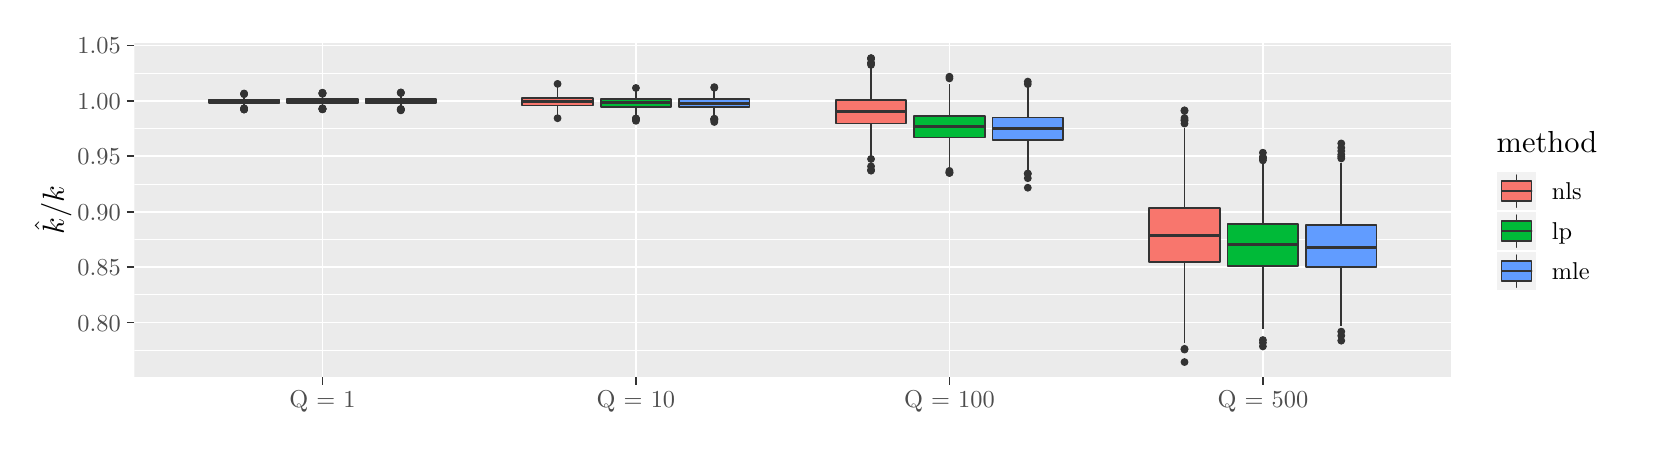
\begin{tikzpicture}[x=1pt,y=1pt]
\definecolor{fillColor}{RGB}{255,255,255}
\path[use as bounding box,fill=fillColor,fill opacity=0.00] (0,0) rectangle (578.16,144.54);
\begin{scope}
\path[clip] (  0.00,  0.00) rectangle (578.16,144.54);
\definecolor{drawColor}{RGB}{255,255,255}
\definecolor{fillColor}{RGB}{255,255,255}

\path[draw=drawColor,line width= 0.6pt,line join=round,line cap=round,fill=fillColor] (  0.00,  0.00) rectangle (578.16,144.54);
\end{scope}
\begin{scope}
\path[clip] ( 38.56, 18.22) rectangle (514.31,139.04);
\definecolor{fillColor}{gray}{0.92}

\path[fill=fillColor] ( 38.56, 18.22) rectangle (514.31,139.04);
\definecolor{drawColor}{RGB}{255,255,255}

\path[draw=drawColor,line width= 0.3pt,line join=round] ( 38.56, 27.95) --
	(514.31, 27.95);

\path[draw=drawColor,line width= 0.3pt,line join=round] ( 38.56, 47.98) --
	(514.31, 47.98);

\path[draw=drawColor,line width= 0.3pt,line join=round] ( 38.56, 68.01) --
	(514.31, 68.01);

\path[draw=drawColor,line width= 0.3pt,line join=round] ( 38.56, 88.03) --
	(514.31, 88.03);

\path[draw=drawColor,line width= 0.3pt,line join=round] ( 38.56,108.06) --
	(514.31,108.06);

\path[draw=drawColor,line width= 0.3pt,line join=round] ( 38.56,128.09) --
	(514.31,128.09);

\path[draw=drawColor,line width= 0.6pt,line join=round] ( 38.56, 37.96) --
	(514.31, 37.96);

\path[draw=drawColor,line width= 0.6pt,line join=round] ( 38.56, 57.99) --
	(514.31, 57.99);

\path[draw=drawColor,line width= 0.6pt,line join=round] ( 38.56, 78.02) --
	(514.31, 78.02);

\path[draw=drawColor,line width= 0.6pt,line join=round] ( 38.56, 98.05) --
	(514.31, 98.05);

\path[draw=drawColor,line width= 0.6pt,line join=round] ( 38.56,118.08) --
	(514.31,118.08);

\path[draw=drawColor,line width= 0.6pt,line join=round] ( 38.56,138.11) --
	(514.31,138.11);

\path[draw=drawColor,line width= 0.6pt,line join=round] (106.52, 18.22) --
	(106.52,139.04);

\path[draw=drawColor,line width= 0.6pt,line join=round] (219.79, 18.22) --
	(219.79,139.04);

\path[draw=drawColor,line width= 0.6pt,line join=round] (333.07, 18.22) --
	(333.07,139.04);

\path[draw=drawColor,line width= 0.6pt,line join=round] (446.34, 18.22) --
	(446.34,139.04);
\definecolor{drawColor}{gray}{0.20}
\definecolor{fillColor}{gray}{0.20}

\path[draw=drawColor,line width= 0.4pt,line join=round,line cap=round,fill=fillColor] ( 78.20,114.98) circle (  1.21);

\path[draw=drawColor,line width= 0.4pt,line join=round,line cap=round,fill=fillColor] ( 78.20,115.34) circle (  1.21);

\path[draw=drawColor,line width= 0.4pt,line join=round,line cap=round,fill=fillColor] ( 78.20,115.07) circle (  1.21);

\path[draw=drawColor,line width= 0.4pt,line join=round,line cap=round,fill=fillColor] ( 78.20,120.60) circle (  1.21);

\path[draw=drawColor,line width= 0.4pt,line join=round,line cap=round,fill=fillColor] ( 78.20,115.40) circle (  1.21);

\path[draw=drawColor,line width= 0.4pt,line join=round,line cap=round,fill=fillColor] ( 78.20,120.76) circle (  1.21);

\path[draw=drawColor,line width= 0.4pt,line join=round,line cap=round,fill=fillColor] ( 78.20,114.98) circle (  1.21);

\path[draw=drawColor,line width= 0.4pt,line join=round,line cap=round,fill=fillColor] ( 78.20,120.51) circle (  1.21);

\path[draw=drawColor,line width= 0.4pt,line join=round,line cap=round,fill=fillColor] ( 78.20,115.17) circle (  1.21);

\path[draw=drawColor,line width= 0.6pt,line join=round] ( 78.20,118.58) -- ( 78.20,120.45);

\path[draw=drawColor,line width= 0.6pt,line join=round] ( 78.20,117.33) -- ( 78.20,115.54);
\definecolor{fillColor}{RGB}{248,118,109}

\path[draw=drawColor,line width= 0.6pt,line join=round,line cap=round,fill=fillColor] ( 65.46,118.58) --
	( 65.46,117.33) --
	( 90.94,117.33) --
	( 90.94,118.58) --
	( 65.46,118.58) --
	cycle;

\path[draw=drawColor,line width= 1.1pt,line join=round] ( 65.46,117.96) -- ( 90.94,117.96);
\definecolor{fillColor}{gray}{0.20}

\path[draw=drawColor,line width= 0.4pt,line join=round,line cap=round,fill=fillColor] (106.52,120.68) circle (  1.21);

\path[draw=drawColor,line width= 0.4pt,line join=round,line cap=round,fill=fillColor] (106.52,115.11) circle (  1.21);

\path[draw=drawColor,line width= 0.4pt,line join=round,line cap=round,fill=fillColor] (106.52,115.01) circle (  1.21);

\path[draw=drawColor,line width= 0.4pt,line join=round,line cap=round,fill=fillColor] (106.52,115.38) circle (  1.21);

\path[draw=drawColor,line width= 0.4pt,line join=round,line cap=round,fill=fillColor] (106.52,115.29) circle (  1.21);

\path[draw=drawColor,line width= 0.4pt,line join=round,line cap=round,fill=fillColor] (106.52,120.67) circle (  1.21);

\path[draw=drawColor,line width= 0.4pt,line join=round,line cap=round,fill=fillColor] (106.52,121.05) circle (  1.21);

\path[draw=drawColor,line width= 0.4pt,line join=round,line cap=round,fill=fillColor] (106.52,120.94) circle (  1.21);

\path[draw=drawColor,line width= 0.4pt,line join=round,line cap=round,fill=fillColor] (106.52,115.28) circle (  1.21);

\path[draw=drawColor,line width= 0.4pt,line join=round,line cap=round,fill=fillColor] (106.52,120.87) circle (  1.21);

\path[draw=drawColor,line width= 0.4pt,line join=round,line cap=round,fill=fillColor] (106.52,115.07) circle (  1.21);

\path[draw=drawColor,line width= 0.6pt,line join=round] (106.52,118.66) -- (106.52,120.58);

\path[draw=drawColor,line width= 0.6pt,line join=round] (106.52,117.35) -- (106.52,115.40);
\definecolor{fillColor}{RGB}{0,186,56}

\path[draw=drawColor,line width= 0.6pt,line join=round,line cap=round,fill=fillColor] ( 93.78,118.66) --
	( 93.78,117.35) --
	(119.26,117.35) --
	(119.26,118.66) --
	( 93.78,118.66) --
	cycle;

\path[draw=drawColor,line width= 1.1pt,line join=round] ( 93.78,118.02) -- (119.26,118.02);
\definecolor{fillColor}{gray}{0.20}

\path[draw=drawColor,line width= 0.4pt,line join=round,line cap=round,fill=fillColor] (134.84,114.66) circle (  1.21);

\path[draw=drawColor,line width= 0.4pt,line join=round,line cap=round,fill=fillColor] (134.84,115.16) circle (  1.21);

\path[draw=drawColor,line width= 0.4pt,line join=round,line cap=round,fill=fillColor] (134.84,114.83) circle (  1.21);

\path[draw=drawColor,line width= 0.4pt,line join=round,line cap=round,fill=fillColor] (134.84,115.03) circle (  1.21);

\path[draw=drawColor,line width= 0.4pt,line join=round,line cap=round,fill=fillColor] (134.84,121.15) circle (  1.21);

\path[draw=drawColor,line width= 0.4pt,line join=round,line cap=round,fill=fillColor] (134.84,120.92) circle (  1.21);

\path[draw=drawColor,line width= 0.4pt,line join=round,line cap=round,fill=fillColor] (134.84,121.02) circle (  1.21);

\path[draw=drawColor,line width= 0.4pt,line join=round,line cap=round,fill=fillColor] (134.84,115.04) circle (  1.21);

\path[draw=drawColor,line width= 0.6pt,line join=round] (134.84,118.71) -- (134.84,120.71);

\path[draw=drawColor,line width= 0.6pt,line join=round] (134.84,117.31) -- (134.84,115.32);
\definecolor{fillColor}{RGB}{97,156,255}

\path[draw=drawColor,line width= 0.6pt,line join=round,line cap=round,fill=fillColor] (122.09,118.71) --
	(122.09,117.31) --
	(147.58,117.31) --
	(147.58,118.71) --
	(122.09,118.71) --
	cycle;

\path[draw=drawColor,line width= 1.1pt,line join=round] (122.09,118.01) -- (147.58,118.01);
\definecolor{fillColor}{gray}{0.20}

\path[draw=drawColor,line width= 0.4pt,line join=round,line cap=round,fill=fillColor] (191.48,124.23) circle (  1.21);

\path[draw=drawColor,line width= 0.4pt,line join=round,line cap=round,fill=fillColor] (191.48,111.82) circle (  1.21);

\path[draw=drawColor,line width= 0.6pt,line join=round] (191.48,119.18) -- (191.48,123.29);

\path[draw=drawColor,line width= 0.6pt,line join=round] (191.48,116.37) -- (191.48,112.30);
\definecolor{fillColor}{RGB}{248,118,109}

\path[draw=drawColor,line width= 0.6pt,line join=round,line cap=round,fill=fillColor] (178.73,119.18) --
	(178.73,116.37) --
	(204.22,116.37) --
	(204.22,119.18) --
	(178.73,119.18) --
	cycle;

\path[draw=drawColor,line width= 1.1pt,line join=round] (178.73,117.92) -- (204.22,117.92);
\definecolor{fillColor}{gray}{0.20}

\path[draw=drawColor,line width= 0.4pt,line join=round,line cap=round,fill=fillColor] (219.79,111.26) circle (  1.21);

\path[draw=drawColor,line width= 0.4pt,line join=round,line cap=round,fill=fillColor] (219.79,111.66) circle (  1.21);

\path[draw=drawColor,line width= 0.4pt,line join=round,line cap=round,fill=fillColor] (219.79,111.70) circle (  1.21);

\path[draw=drawColor,line width= 0.4pt,line join=round,line cap=round,fill=fillColor] (219.79,122.75) circle (  1.21);

\path[draw=drawColor,line width= 0.4pt,line join=round,line cap=round,fill=fillColor] (219.79,111.65) circle (  1.21);

\path[draw=drawColor,line width= 0.4pt,line join=round,line cap=round,fill=fillColor] (219.79,110.88) circle (  1.21);

\path[draw=drawColor,line width= 0.6pt,line join=round] (219.79,118.68) -- (219.79,122.72);

\path[draw=drawColor,line width= 0.6pt,line join=round] (219.79,115.98) -- (219.79,111.95);
\definecolor{fillColor}{RGB}{0,186,56}

\path[draw=drawColor,line width= 0.6pt,line join=round,line cap=round,fill=fillColor] (207.05,118.68) --
	(207.05,115.98) --
	(232.54,115.98) --
	(232.54,118.68) --
	(207.05,118.68) --
	cycle;

\path[draw=drawColor,line width= 1.1pt,line join=round] (207.05,117.33) -- (232.54,117.33);
\definecolor{fillColor}{gray}{0.20}

\path[draw=drawColor,line width= 0.4pt,line join=round,line cap=round,fill=fillColor] (248.11,110.46) circle (  1.21);

\path[draw=drawColor,line width= 0.4pt,line join=round,line cap=round,fill=fillColor] (248.11,111.49) circle (  1.21);

\path[draw=drawColor,line width= 0.4pt,line join=round,line cap=round,fill=fillColor] (248.11,111.63) circle (  1.21);

\path[draw=drawColor,line width= 0.4pt,line join=round,line cap=round,fill=fillColor] (248.11,111.38) circle (  1.21);

\path[draw=drawColor,line width= 0.4pt,line join=round,line cap=round,fill=fillColor] (248.11,122.84) circle (  1.21);

\path[draw=drawColor,line width= 0.4pt,line join=round,line cap=round,fill=fillColor] (248.11,111.55) circle (  1.21);

\path[draw=drawColor,line width= 0.4pt,line join=round,line cap=round,fill=fillColor] (248.11,110.95) circle (  1.21);

\path[draw=drawColor,line width= 0.4pt,line join=round,line cap=round,fill=fillColor] (248.11,123.06) circle (  1.21);

\path[draw=drawColor,line width= 0.6pt,line join=round] (248.11,118.65) -- (248.11,122.72);

\path[draw=drawColor,line width= 0.6pt,line join=round] (248.11,115.91) -- (248.11,111.86);
\definecolor{fillColor}{RGB}{97,156,255}

\path[draw=drawColor,line width= 0.6pt,line join=round,line cap=round,fill=fillColor] (235.37,118.65) --
	(235.37,115.91) --
	(260.86,115.91) --
	(260.86,118.65) --
	(235.37,118.65) --
	cycle;

\path[draw=drawColor,line width= 1.1pt,line join=round] (235.37,117.26) -- (260.86,117.26);
\definecolor{fillColor}{gray}{0.20}

\path[draw=drawColor,line width= 0.4pt,line join=round,line cap=round,fill=fillColor] (304.75,131.80) circle (  1.21);

\path[draw=drawColor,line width= 0.4pt,line join=round,line cap=round,fill=fillColor] (304.75,131.10) circle (  1.21);

\path[draw=drawColor,line width= 0.4pt,line join=round,line cap=round,fill=fillColor] (304.75,133.32) circle (  1.21);

\path[draw=drawColor,line width= 0.4pt,line join=round,line cap=round,fill=fillColor] (304.75,133.55) circle (  1.21);

\path[draw=drawColor,line width= 0.4pt,line join=round,line cap=round,fill=fillColor] (304.75, 94.44) circle (  1.21);

\path[draw=drawColor,line width= 0.4pt,line join=round,line cap=round,fill=fillColor] (304.75, 93.16) circle (  1.21);

\path[draw=drawColor,line width= 0.4pt,line join=round,line cap=round,fill=fillColor] (304.75,133.39) circle (  1.21);

\path[draw=drawColor,line width= 0.4pt,line join=round,line cap=round,fill=fillColor] (304.75,131.73) circle (  1.21);

\path[draw=drawColor,line width= 0.4pt,line join=round,line cap=round,fill=fillColor] (304.75, 92.87) circle (  1.21);

\path[draw=drawColor,line width= 0.4pt,line join=round,line cap=round,fill=fillColor] (304.75, 97.09) circle (  1.21);

\path[draw=drawColor,line width= 0.6pt,line join=round] (304.75,118.33) -- (304.75,130.87);

\path[draw=drawColor,line width= 0.6pt,line join=round] (304.75,109.87) -- (304.75, 97.88);
\definecolor{fillColor}{RGB}{248,118,109}

\path[draw=drawColor,line width= 0.6pt,line join=round,line cap=round,fill=fillColor] (292.01,118.33) --
	(292.01,109.87) --
	(317.49,109.87) --
	(317.49,118.33) --
	(292.01,118.33) --
	cycle;

\path[draw=drawColor,line width= 1.1pt,line join=round] (292.01,114.26) -- (317.49,114.26);
\definecolor{fillColor}{gray}{0.20}

\path[draw=drawColor,line width= 0.4pt,line join=round,line cap=round,fill=fillColor] (333.07,126.19) circle (  1.21);

\path[draw=drawColor,line width= 0.4pt,line join=round,line cap=round,fill=fillColor] (333.07, 92.06) circle (  1.21);

\path[draw=drawColor,line width= 0.4pt,line join=round,line cap=round,fill=fillColor] (333.07, 92.32) circle (  1.21);

\path[draw=drawColor,line width= 0.4pt,line join=round,line cap=round,fill=fillColor] (333.07,126.81) circle (  1.21);

\path[draw=drawColor,line width= 0.4pt,line join=round,line cap=round,fill=fillColor] (333.07, 92.78) circle (  1.21);

\path[draw=drawColor,line width= 0.4pt,line join=round,line cap=round,fill=fillColor] (333.07, 92.05) circle (  1.21);

\path[draw=drawColor,line width= 0.6pt,line join=round] (333.07,112.74) -- (333.07,124.08);

\path[draw=drawColor,line width= 0.6pt,line join=round] (333.07,104.84) -- (333.07, 93.24);
\definecolor{fillColor}{RGB}{0,186,56}

\path[draw=drawColor,line width= 0.6pt,line join=round,line cap=round,fill=fillColor] (320.33,112.74) --
	(320.33,104.84) --
	(345.81,104.84) --
	(345.81,112.74) --
	(320.33,112.74) --
	cycle;

\path[draw=drawColor,line width= 1.1pt,line join=round] (320.33,108.87) -- (345.81,108.87);
\definecolor{fillColor}{gray}{0.20}

\path[draw=drawColor,line width= 0.4pt,line join=round,line cap=round,fill=fillColor] (361.39, 91.84) circle (  1.21);

\path[draw=drawColor,line width= 0.4pt,line join=round,line cap=round,fill=fillColor] (361.39,125.05) circle (  1.21);

\path[draw=drawColor,line width= 0.4pt,line join=round,line cap=round,fill=fillColor] (361.39, 86.70) circle (  1.21);

\path[draw=drawColor,line width= 0.4pt,line join=round,line cap=round,fill=fillColor] (361.39, 91.74) circle (  1.21);

\path[draw=drawColor,line width= 0.4pt,line join=round,line cap=round,fill=fillColor] (361.39,124.15) circle (  1.21);

\path[draw=drawColor,line width= 0.4pt,line join=round,line cap=round,fill=fillColor] (361.39, 90.16) circle (  1.21);

\path[draw=drawColor,line width= 0.6pt,line join=round] (361.39,112.07) -- (361.39,123.78);

\path[draw=drawColor,line width= 0.6pt,line join=round] (361.39,104.02) -- (361.39, 92.23);
\definecolor{fillColor}{RGB}{97,156,255}

\path[draw=drawColor,line width= 0.6pt,line join=round,line cap=round,fill=fillColor] (348.64,112.07) --
	(348.64,104.02) --
	(374.13,104.02) --
	(374.13,112.07) --
	(348.64,112.07) --
	cycle;

\path[draw=drawColor,line width= 1.1pt,line join=round] (348.64,108.02) -- (374.13,108.02);
\definecolor{fillColor}{gray}{0.20}

\path[draw=drawColor,line width= 0.4pt,line join=round,line cap=round,fill=fillColor] (418.02,114.68) circle (  1.21);

\path[draw=drawColor,line width= 0.4pt,line join=round,line cap=round,fill=fillColor] (418.02, 28.49) circle (  1.21);

\path[draw=drawColor,line width= 0.4pt,line join=round,line cap=round,fill=fillColor] (418.02,111.24) circle (  1.21);

\path[draw=drawColor,line width= 0.4pt,line join=round,line cap=round,fill=fillColor] (418.02, 23.71) circle (  1.21);

\path[draw=drawColor,line width= 0.4pt,line join=round,line cap=round,fill=fillColor] (418.02,111.90) circle (  1.21);

\path[draw=drawColor,line width= 0.4pt,line join=round,line cap=round,fill=fillColor] (418.02, 28.22) circle (  1.21);

\path[draw=drawColor,line width= 0.4pt,line join=round,line cap=round,fill=fillColor] (418.02,109.89) circle (  1.21);

\path[draw=drawColor,line width= 0.4pt,line join=round,line cap=round,fill=fillColor] (418.02,110.95) circle (  1.21);

\path[draw=drawColor,line width= 0.4pt,line join=round,line cap=round,fill=fillColor] (418.02,114.46) circle (  1.21);

\path[draw=drawColor,line width= 0.6pt,line join=round] (418.02, 79.39) -- (418.02,108.39);

\path[draw=drawColor,line width= 0.6pt,line join=round] (418.02, 59.81) -- (418.02, 30.56);
\definecolor{fillColor}{RGB}{248,118,109}

\path[draw=drawColor,line width= 0.6pt,line join=round,line cap=round,fill=fillColor] (405.28, 79.39) --
	(405.28, 59.81) --
	(430.77, 59.81) --
	(430.77, 79.39) --
	(405.28, 79.39) --
	cycle;

\path[draw=drawColor,line width= 1.1pt,line join=round] (405.28, 69.57) -- (430.77, 69.57);
\definecolor{fillColor}{gray}{0.20}

\path[draw=drawColor,line width= 0.4pt,line join=round,line cap=round,fill=fillColor] (446.34, 97.75) circle (  1.21);

\path[draw=drawColor,line width= 0.4pt,line join=round,line cap=round,fill=fillColor] (446.34, 99.36) circle (  1.21);

\path[draw=drawColor,line width= 0.4pt,line join=round,line cap=round,fill=fillColor] (446.34, 97.54) circle (  1.21);

\path[draw=drawColor,line width= 0.4pt,line join=round,line cap=round,fill=fillColor] (446.34, 31.66) circle (  1.21);

\path[draw=drawColor,line width= 0.4pt,line join=round,line cap=round,fill=fillColor] (446.34, 30.70) circle (  1.21);

\path[draw=drawColor,line width= 0.4pt,line join=round,line cap=round,fill=fillColor] (446.34, 96.59) circle (  1.21);

\path[draw=drawColor,line width= 0.4pt,line join=round,line cap=round,fill=fillColor] (446.34, 29.37) circle (  1.21);

\path[draw=drawColor,line width= 0.4pt,line join=round,line cap=round,fill=fillColor] (446.34, 97.13) circle (  1.21);

\path[draw=drawColor,line width= 0.4pt,line join=round,line cap=round,fill=fillColor] (446.34, 97.59) circle (  1.21);

\path[draw=drawColor,line width= 0.6pt,line join=round] (446.34, 73.68) -- (446.34, 95.91);

\path[draw=drawColor,line width= 0.6pt,line join=round] (446.34, 58.46) -- (446.34, 35.64);
\definecolor{fillColor}{RGB}{0,186,56}

\path[draw=drawColor,line width= 0.6pt,line join=round,line cap=round,fill=fillColor] (433.60, 73.68) --
	(433.60, 58.46) --
	(459.09, 58.46) --
	(459.09, 73.68) --
	(433.60, 73.68) --
	cycle;

\path[draw=drawColor,line width= 1.1pt,line join=round] (433.60, 66.27) -- (459.09, 66.27);
\definecolor{fillColor}{gray}{0.20}

\path[draw=drawColor,line width= 0.4pt,line join=round,line cap=round,fill=fillColor] (474.66, 97.29) circle (  1.21);

\path[draw=drawColor,line width= 0.4pt,line join=round,line cap=round,fill=fillColor] (474.66, 98.67) circle (  1.21);

\path[draw=drawColor,line width= 0.4pt,line join=round,line cap=round,fill=fillColor] (474.66,101.15) circle (  1.21);

\path[draw=drawColor,line width= 0.4pt,line join=round,line cap=round,fill=fillColor] (474.66, 34.71) circle (  1.21);

\path[draw=drawColor,line width= 0.4pt,line join=round,line cap=round,fill=fillColor] (474.66, 99.97) circle (  1.21);

\path[draw=drawColor,line width= 0.4pt,line join=round,line cap=round,fill=fillColor] (474.66, 31.44) circle (  1.21);

\path[draw=drawColor,line width= 0.4pt,line join=round,line cap=round,fill=fillColor] (474.66, 33.23) circle (  1.21);

\path[draw=drawColor,line width= 0.4pt,line join=round,line cap=round,fill=fillColor] (474.66, 97.94) circle (  1.21);

\path[draw=drawColor,line width= 0.4pt,line join=round,line cap=round,fill=fillColor] (474.66,102.71) circle (  1.21);

\path[draw=drawColor,line width= 0.6pt,line join=round] (474.66, 73.16) -- (474.66, 95.81);

\path[draw=drawColor,line width= 0.6pt,line join=round] (474.66, 58.04) -- (474.66, 36.69);
\definecolor{fillColor}{RGB}{97,156,255}

\path[draw=drawColor,line width= 0.6pt,line join=round,line cap=round,fill=fillColor] (461.92, 73.16) --
	(461.92, 58.04) --
	(487.40, 58.04) --
	(487.40, 73.16) --
	(461.92, 73.16) --
	cycle;

\path[draw=drawColor,line width= 1.1pt,line join=round] (461.92, 65.10) -- (487.40, 65.10);
\end{scope}
\begin{scope}
\path[clip] (  0.00,  0.00) rectangle (578.16,144.54);
\definecolor{drawColor}{gray}{0.30}

\node[text=drawColor,anchor=base east,inner sep=0pt, outer sep=0pt, scale=  0.88] at ( 33.61, 34.93) {0.80};

\node[text=drawColor,anchor=base east,inner sep=0pt, outer sep=0pt, scale=  0.88] at ( 33.61, 54.96) {0.85};

\node[text=drawColor,anchor=base east,inner sep=0pt, outer sep=0pt, scale=  0.88] at ( 33.61, 74.99) {0.90};

\node[text=drawColor,anchor=base east,inner sep=0pt, outer sep=0pt, scale=  0.88] at ( 33.61, 95.02) {0.95};

\node[text=drawColor,anchor=base east,inner sep=0pt, outer sep=0pt, scale=  0.88] at ( 33.61,115.05) {1.00};

\node[text=drawColor,anchor=base east,inner sep=0pt, outer sep=0pt, scale=  0.88] at ( 33.61,135.08) {1.05};
\end{scope}
\begin{scope}
\path[clip] (  0.00,  0.00) rectangle (578.16,144.54);
\definecolor{drawColor}{gray}{0.20}

\path[draw=drawColor,line width= 0.6pt,line join=round] ( 35.81, 37.96) --
	( 38.56, 37.96);

\path[draw=drawColor,line width= 0.6pt,line join=round] ( 35.81, 57.99) --
	( 38.56, 57.99);

\path[draw=drawColor,line width= 0.6pt,line join=round] ( 35.81, 78.02) --
	( 38.56, 78.02);

\path[draw=drawColor,line width= 0.6pt,line join=round] ( 35.81, 98.05) --
	( 38.56, 98.05);

\path[draw=drawColor,line width= 0.6pt,line join=round] ( 35.81,118.08) --
	( 38.56,118.08);

\path[draw=drawColor,line width= 0.6pt,line join=round] ( 35.81,138.11) --
	( 38.56,138.11);
\end{scope}
\begin{scope}
\path[clip] (  0.00,  0.00) rectangle (578.16,144.54);
\definecolor{drawColor}{gray}{0.20}

\path[draw=drawColor,line width= 0.6pt,line join=round] (106.52, 15.47) --
	(106.52, 18.22);

\path[draw=drawColor,line width= 0.6pt,line join=round] (219.79, 15.47) --
	(219.79, 18.22);

\path[draw=drawColor,line width= 0.6pt,line join=round] (333.07, 15.47) --
	(333.07, 18.22);

\path[draw=drawColor,line width= 0.6pt,line join=round] (446.34, 15.47) --
	(446.34, 18.22);
\end{scope}
\begin{scope}
\path[clip] (  0.00,  0.00) rectangle (578.16,144.54);
\definecolor{drawColor}{gray}{0.30}

\node[text=drawColor,anchor=base,inner sep=0pt, outer sep=0pt, scale=  0.88] at (106.52,  7.21) {Q = 1};

\node[text=drawColor,anchor=base,inner sep=0pt, outer sep=0pt, scale=  0.88] at (219.79,  7.21) {Q = 10};

\node[text=drawColor,anchor=base,inner sep=0pt, outer sep=0pt, scale=  0.88] at (333.07,  7.21) {Q = 100};

\node[text=drawColor,anchor=base,inner sep=0pt, outer sep=0pt, scale=  0.88] at (446.34,  7.21) {Q = 500};
\end{scope}
\begin{scope}
\path[clip] (  0.00,  0.00) rectangle (578.16,144.54);
\definecolor{drawColor}{RGB}{0,0,0}

\node[text=drawColor,rotate= 90.00,anchor=base,inner sep=0pt, outer sep=0pt, scale=  1.10] at ( 13.08, 78.63) {$\hat{k}/k$};
\end{scope}
\begin{scope}
\path[clip] (  0.00,  0.00) rectangle (578.16,144.54);
\definecolor{fillColor}{RGB}{255,255,255}

\path[fill=fillColor] (525.31, 43.84) rectangle (572.66,113.42);
\end{scope}
\begin{scope}
\path[clip] (  0.00,  0.00) rectangle (578.16,144.54);
\definecolor{drawColor}{RGB}{0,0,0}

\node[text=drawColor,anchor=base west,inner sep=0pt, outer sep=0pt, scale=  1.10] at (530.81, 99.27) {method};
\end{scope}
\begin{scope}
\path[clip] (  0.00,  0.00) rectangle (578.16,144.54);
\definecolor{drawColor}{RGB}{255,255,255}
\definecolor{fillColor}{gray}{0.95}

\path[draw=drawColor,line width= 0.6pt,line join=round,line cap=round,fill=fillColor] (530.81, 78.25) rectangle (545.26, 92.70);
\end{scope}
\begin{scope}
\path[clip] (  0.00,  0.00) rectangle (578.16,144.54);
\definecolor{drawColor}{gray}{0.20}

\path[draw=drawColor,line width= 0.6pt,line join=round,line cap=round] (538.03, 79.70) --
	(538.03, 81.86);

\path[draw=drawColor,line width= 0.6pt,line join=round,line cap=round] (538.03, 89.09) --
	(538.03, 91.26);
\definecolor{fillColor}{RGB}{248,118,109}

\path[draw=drawColor,line width= 0.6pt,line join=round,line cap=round,fill=fillColor] (532.61, 81.86) rectangle (543.45, 89.09);

\path[draw=drawColor,line width= 0.6pt,line join=round,line cap=round] (532.61, 85.48) --
	(543.45, 85.48);
\end{scope}
\begin{scope}
\path[clip] (  0.00,  0.00) rectangle (578.16,144.54);
\definecolor{drawColor}{RGB}{255,255,255}
\definecolor{fillColor}{gray}{0.95}

\path[draw=drawColor,line width= 0.6pt,line join=round,line cap=round,fill=fillColor] (530.81, 63.80) rectangle (545.26, 78.25);
\end{scope}
\begin{scope}
\path[clip] (  0.00,  0.00) rectangle (578.16,144.54);
\definecolor{drawColor}{gray}{0.20}

\path[draw=drawColor,line width= 0.6pt,line join=round,line cap=round] (538.03, 65.24) --
	(538.03, 67.41);

\path[draw=drawColor,line width= 0.6pt,line join=round,line cap=round] (538.03, 74.64) --
	(538.03, 76.81);
\definecolor{fillColor}{RGB}{0,186,56}

\path[draw=drawColor,line width= 0.6pt,line join=round,line cap=round,fill=fillColor] (532.61, 67.41) rectangle (543.45, 74.64);

\path[draw=drawColor,line width= 0.6pt,line join=round,line cap=round] (532.61, 71.02) --
	(543.45, 71.02);
\end{scope}
\begin{scope}
\path[clip] (  0.00,  0.00) rectangle (578.16,144.54);
\definecolor{drawColor}{RGB}{255,255,255}
\definecolor{fillColor}{gray}{0.95}

\path[draw=drawColor,line width= 0.6pt,line join=round,line cap=round,fill=fillColor] (530.81, 49.34) rectangle (545.26, 63.80);
\end{scope}
\begin{scope}
\path[clip] (  0.00,  0.00) rectangle (578.16,144.54);
\definecolor{drawColor}{gray}{0.20}

\path[draw=drawColor,line width= 0.6pt,line join=round,line cap=round] (538.03, 50.79) --
	(538.03, 52.96);

\path[draw=drawColor,line width= 0.6pt,line join=round,line cap=round] (538.03, 60.18) --
	(538.03, 62.35);
\definecolor{fillColor}{RGB}{97,156,255}

\path[draw=drawColor,line width= 0.6pt,line join=round,line cap=round,fill=fillColor] (532.61, 52.96) rectangle (543.45, 60.18);

\path[draw=drawColor,line width= 0.6pt,line join=round,line cap=round] (532.61, 56.57) --
	(543.45, 56.57);
\end{scope}
\begin{scope}
\path[clip] (  0.00,  0.00) rectangle (578.16,144.54);
\definecolor{drawColor}{RGB}{0,0,0}

\node[text=drawColor,anchor=base west,inner sep=0pt, outer sep=0pt, scale=  0.88] at (550.76, 82.45) {nls};
\end{scope}
\begin{scope}
\path[clip] (  0.00,  0.00) rectangle (578.16,144.54);
\definecolor{drawColor}{RGB}{0,0,0}

\node[text=drawColor,anchor=base west,inner sep=0pt, outer sep=0pt, scale=  0.88] at (550.76, 67.99) {lp};
\end{scope}
\begin{scope}
\path[clip] (  0.00,  0.00) rectangle (578.16,144.54);
\definecolor{drawColor}{RGB}{0,0,0}

\node[text=drawColor,anchor=base west,inner sep=0pt, outer sep=0pt, scale=  0.88] at (550.76, 53.54) {mle};
\end{scope}
\end{tikzpicture}
